\documentclass[12pt]{article}

\usepackage[margin=0.8 in]{geometry}
\usepackage{amsmath}
\usepackage{amssymb}
\usepackage{macros}
\usepackage{mathtools}
\usepackage{enumerate}
\usepackage{verbatim}
\usepackage{amsthm}

\title{}
%\content{}



\let \proj \undefined
\renewcommand{\tr}{ \mathrm{tr}}
\DeclareMathOperator{\SU}{SU}
\DeclareMathOperator{\proj}{proj}
\newcommand{\sS}{\mathscr{S}}
\DeclareMathOperator{\comp}{comp}
\newcommand{\A}{\mathcal{A}}
\renewcommand{\D}{\mathcal{D}}
\renewcommand{\e}{\epsilon}
\newcommand{\Are}{\A_{r,\e}}
\newcommand{\Kre}{K_{r,\e}}
\newcommand{\Dre}{\D_{r,\e}}
\newcommand{\rt}{\tilde{r}}
\newcommand{\et}{\tilde{\e}}
\newtheorem{definition}{Definition}
\newenvironment{solution}
  {\begin{proof}[Solution]}
  {\end{proof}}
\newtheorem{example}{Example}
\newtheorem{exercise}{Exercise}

\newcommand{\vr}{\mathbf{r}}
\newcommand{\vF}{\mathbf{F}}

\newtheorem{theorem}{Theorem}



\begin{document}
\section*{15.4 Polar Coordinates}
Goals from this section
\begin{enumerate}
\item Know how to rewrite Cartesian coordinates to polar and vice versa
\item Be able to integrate in polar coordinates
\item It might be good for you to remember the value of the Gaussian integral, though you don't have to for this class.
\end{enumerate}
\textbf{Motivation: } As you might already have noticed, some objects are easier to express in $x$, $y$ (Cartesian) coordinates. For example, the line $y=2$ is easy to describe because the distance of each point from the $x$ axis is always constant. Now if we look at a circle centered at the origin, we see that the expression is slightly more complicated: $x^2+y^2=r^2$. The distance of its points from any of the axes is not constant, however the distance of its points from the origin is constant. Similarly, the half line $y=\sqrt{3}x$, $x\geq 0$, has the property that the line segment connecting any of its points with the origin forms a constant angle of $\frac{\pi}{3}$ with the positive $x$-axis. We will construct a coordinate system engineered to make such objects easily described.

\subsection*{From Cartesian to Polar and back}
We'd like to describe a point $P(x,y)$ on the plane by two numbers $(r,\theta)$ that such that $r$ is its distance from the origin if $r$ is non-negative (that is, the length of $OP$), and $\theta$ is the counter-clockwise angle between the positive $x$-axis and the vector $\vec{OP}$, if $\theta\in [0,\2\pi]$. A reasonable thing to do this is to demand that \begin{equation}
x=r\cos(\theta)
\end{equation}\begin{equation}
y=r\sin(\theta),
\end{equation}
which makes sense if we look at the picture below, and also implies \begin{equation}\label{first}r^2=x^2+y^2\end{equation} and \begin{equation}
\tan(\theta)=\frac{y}{x}.
\end{equation} Note that this allows $r$ to be negative, and $\theta$ to be any real number. In fact, in polar coordinates, $(r,\theta)=(-r,\theta+\pi)$ and $(r,\theta)=(r,\theta + 2k\pi) $ for any integer $k$. Because this introduces too much ambiguity for us to feel comfortable, we usually assume $r\geq 0$ and $\theta\in [0,2\pi)$. This allows us to rewrite \eqref{first} as \begin{equation}
r=\sqrt{x^2+y^2.}
\end{equation}
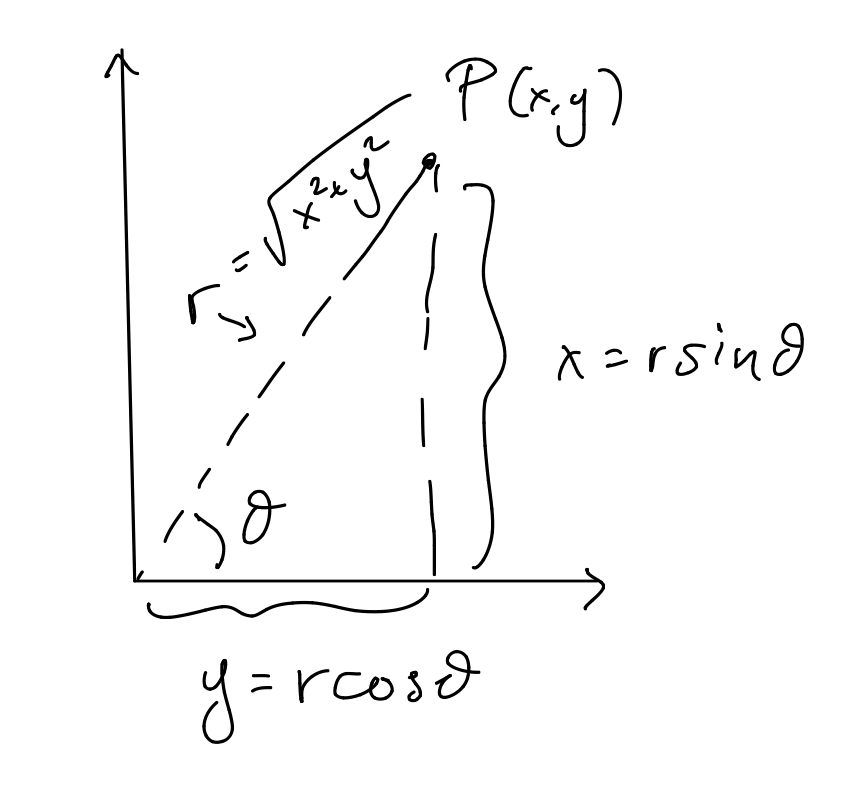
\includegraphics[scale=.2]{polar.jpeg}

\begin{example}The circle centered at the origin with radius $r_0$ can be written as $r=r_0$ in polar coordinates.
\end{example}
\begin{example} Express the disk $(y-2)^2+x^2\leq 4$ in polar coordinates (assuming $r\geq 0$). 
\end{example}
\begin{solution} We have $(r\sin(\theta)-2)^2+r^2\cos^2(\theta)\leq 4$ which gives, after expanding the square, $r^2\leq 4r\sin(\theta)$. If $r\neq 0$ we find \begin{equation}\label{second}r\leq 4\sin(\theta).\end{equation} The case $r=0$ is not really a problem, since in our disk $y=r\sin(\theta)\geq 0\implies \sin(\theta)\geq 0$ so  \eqref{second} still holds. By looking at the picture, we find that $$\theta\in[0,\pi],$$ so we may finally write $$D=\{(r,\theta):0\leq r\leq 4\sin(\theta),0\leq\theta\leq \pi\}.$$
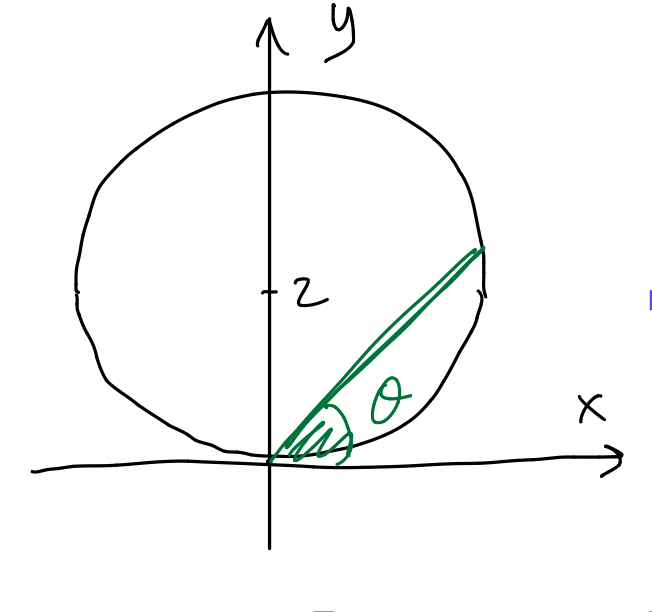
\includegraphics[scale=.2]{disk.jpeg}
\end{solution}

\begin{example} The expression $\theta = \theta_0$ represents a half ray starting at the origin and forming angle $\theta_0$ with the positive $x$ axis.
\end{example}
\begin{example} In figures 1 and 2 you can see a bear under polar transformation:

\begin{figure}
\centering
\parbox{5cm}{
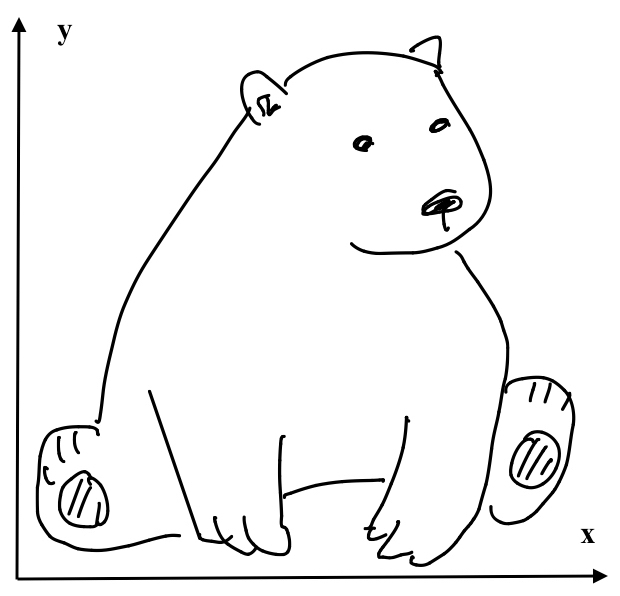
\includegraphics[scale=.2]{cartesian_bear_with_axes.jpeg}
\caption{A Cartesian Bear}}
\label{cartesianbear}
\qquad
\begin{minipage}{5cm}
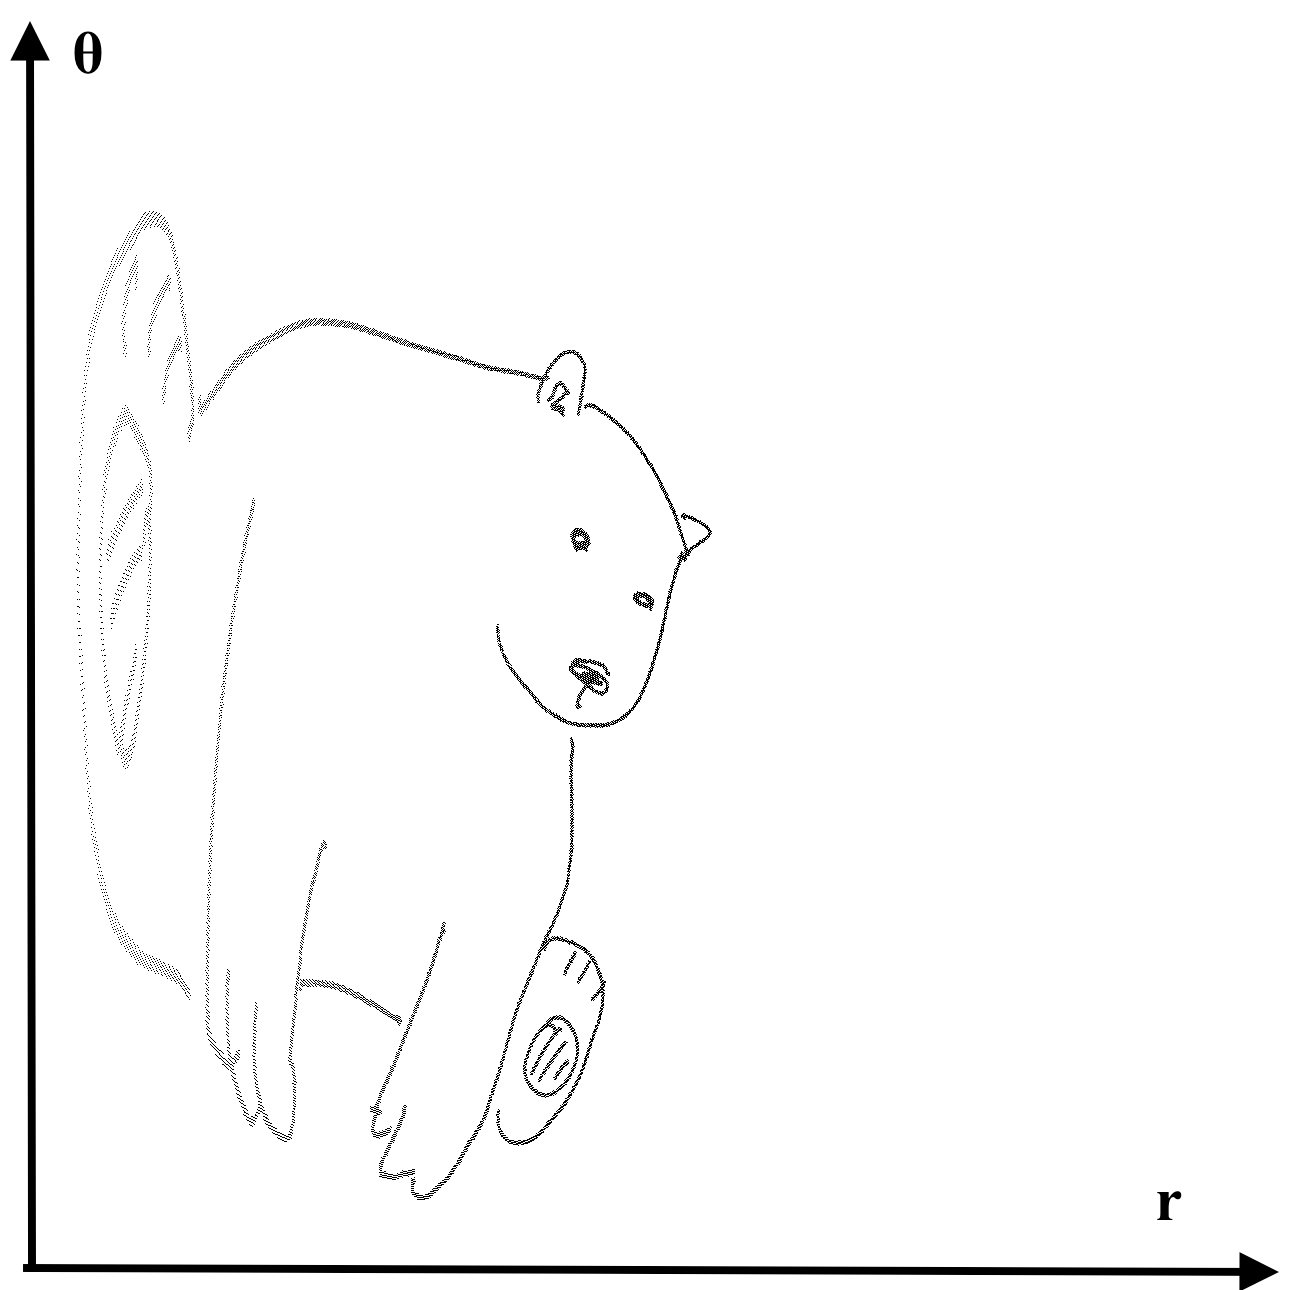
\includegraphics[scale=.1]{polar_bear.png}
\caption{A Polar Bear}
\label{polarbear}
\end{minipage}
\end{figure}







\end{example}

\begin{exercise}How would you write the line $y=2 $ in polar coordinates?
\end{exercise}

\subsection*{Integration in polar coordinates}
\begin{theorem}
Suppose we want to integrate over a domain written as $$D=\{(r,\theta):h_1(\theta)\leq r \leq h_2(\theta), \alpha\leq \theta \leq \beta\}.$$ Then, for a continuous function $f(x,y)$ we have $$\iint_Df(x,y) dA=\int_\alpha^\beta\int_{h_1(\theta)}^{h_2(\theta)}f(r\cos(\theta),r\sin(\theta))r dr d\theta.$$
\end{theorem}

\textbf{Remarks:}\begin{enumerate}
\item Don't forget the $r$ inside the integral!
\item Once you set up the integral in polar coordinates, there must be only $r$ and $\theta$ in your expression, not $x$ and $y$.
\item Polar coordinates are useful when the expression $x^2+y^2$ appears in our function or when the domain of integration can be described easily in polar coordinates, like disks centered at the origin, annuli, sectors of disks etc.
\end{enumerate}


\begin{example}
Set up the integral $\iint_R 2x-y dA$ in polar coordinates, where $R$ is enclosed by $x^2+y^2=4$, $x=0$, $y=x$ in the first quadrant.
\end{example}
\begin{solution} The given domain can be described as $R=\{(r,\theta):0\leq r\leq 2, 0\leq \theta\leq \pi/4\}$, so $$\iint_R 2x-y dA=\int_0^{\frac{\pi}{4}}\int_0^2(2r\cos(\theta)-r\sin(\theta))rdrd
\theta.$$
\end{solution}


\subsection*{An impressive application of polar coordinates: The Gaussian Integral}
We will calculate the integral $\int_{-\infty}^\infty e^{-x^2}dx$. The indefinite integral $\int e^{-x^2}dx$ can't be written in terms of elementary functions, but polar coordinates can help us find $\int_{-\infty}^\infty e^{-x^2}dx$.

Recall that $$\int_{-\infty}^\infty e^{-x^2}dx=\lim_{M\to\infty}\int_{-M}^Me^{-x^2}dx.$$ So let's call $I:=\int_{-\infty}^\infty e^{-x^2}dx$ and $I_M:=\int_{-M}^Me^{-x^2}dx$ so that $I=\lim_{M\to\infty}I_M$.

Let's denote by $R_M:=\{(x,y):|x|\leq M,|y|\leq M\}$ the square of side $2M$ (with its interior), and since $x$ is a dummy variable in the expression for $I_M$, we may write
\begin{align*}
I_M^2=&I_M\cdot I_M\\
=&(\int_{-M}^Me^{-x^2}dx)(\int_{-M}^Me^{-x^2}dx)\\
=&(\int_{-M}^Me^{-x^2}dx)(\int_{-M}^Me^{-y^2}dy)\\
=&\int_{-M}^M\int_{-M}^Me^{-x^2}e^{-y^2}dxdy\\
=&\iint_{R_M}e^{-(x^2+y^2)}dA
\end{align*}

Remember that $x^2+y^2$ is an expression that is easily described in polar coordinates, but the integration is happening on a square, which is not that nice of a situation. So we'll use the \textbf{Sandwich theorem} from elementary calculus that says that if\begin{itemize}
\item $a_M\leq I_M\leq A_M$ for all $M$ and 
\item $\lim_{M\to\infty}a_M=\lim_{M\to \infty}A_M=C$ 
\end{itemize}
then $\lim_{M\to \infty}I_M=C$.  We will try to find appropriate $a_M$ and $A_M$.

Note that if $D_M$ is the disk centered at the origin with radius $M$ and $D_{\sqrt{2}M}$ is the disk centered at the origin with radius ${\sqrt{2}M}$ then we have $$D_M\subset R_M\subset D_{\sqrt{2}M}.$$

Therefore, by Exercise 2 from 15.3 (lecture notes), using that $e^{-(x^2+y^2)}\geq 0$ everywhere, we find that \begin{equation}\label{polar}
\int_{D_M}e^{-(x^2+y^2)}dA\leq \iint_{R_M}e^{-(x^2+y^2)}dA\leq \iint_{D_{\sqrt{2}M}}e^{-(x^2+y^2)}dA.
\end{equation}

Things are starting to look good! Let's see why: Using polar coordinates, \begin{align*}a_M:=&\iint_{D_M}e^{-(x^2+y^2)}dA\\
=& \int_0^{2\pi}\int_0^Me^{-r^2}rdrd\theta\\
=& 2\pi[\frac{-e^{-r^2}}{2}]_0^M\\
=& \pi (1-e^{-M^2})
\end{align*}
so that $\lim_{M\to \infty}a_M=\pi$. As you can check yourself, for $A_M:=\iint_{D_{\sqrt{2}M}}e^{-(x^2+y^2)}dA$, we also find $\lim_{M\to \infty}A_M=\pi$, so by \eqref{polar} and the Sandwich Theorem we find that $$\lim_{M\to \infty}I_M^2=\pi$$ which implies $$I=\int_{-\infty}^\infty e^{-x^2}dx=\sqrt{\pi}.$$
\end{document}

